\usecaseristoratore{Visualizzazione notifica di avvenuto pagamento}
\label{usecase:Visualizzazione notifica di avvenuto pagamento}

\begin{figure}[h]
	\centering
	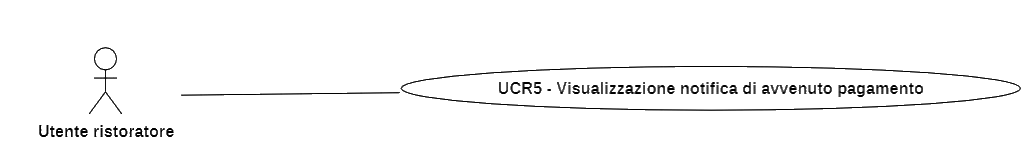
\includegraphics[width=0.9\textwidth]{./uml/UCR5.png} 
	\caption{Visualizzazione notifica di avvenuto pagamento}
	\label{fig:UCR5}
  \end{figure}

\begin{itemize}
	\item \textbf{Attore principale:} Utente ristoratore.

	\item \textbf{Precondizione:} L'Utente base ha effettuato il pagamento del suo conto (vedi \autoref{usecase:Pagamento del conto}).


	\item \textbf{Postcondizione:} L'Utente ristoratore visualizza la notifica
		dell'avvenuto pagamento da parte dell'Utente base.

	\item \textbf{Scenario principale:}
	      \begin{enumerate}
		      \item Il Sistema vede che il pagamento da parte dell'Utente base è andato a buon fine;
		      \item Il Sistema invia all'Utente ristoratore una notifica dell'avvenuto pagamento;
		      \item L'Utente ristoratore visualizza la notifica dell'avvenuto
		            pagamento da parte dell'Utente base.
	      \end{enumerate}
\end{itemize}
